\subsection{Descrição de \textit{software}}\label{subsec:software}

O software funciona como uma estação meteorológica baseada no sensor BME280, integrada a um Raspberry Pi através de comunicação I2C. O processo inicia com a inicialização do barramento e a calibração do sensor, realizando leituras periódicas em uma thread dedicada para não bloquear o servidor web. Os dados coletados passam por validação, sendo posteriormente enviados para um sistema de inteligência artificial em desenvolvimento, responsável por análises preditivas e detecção de padrões climáticos. O sistema mantém os últimos valores em cache, registra logs de eventos e erros, e expõe uma API REST em JSON, facilitando a integração com aplicações externas. 

Além disso, conta com um dashboard web desenvolvido em HTML5, CSS e JavaScript, permitindo ao usuário visualizar informações e a coleta de dados. A aplicação é executada como um serviço systemd, configurado para iniciar automaticamente. Por fim, sua arquitetura é baseada em threads, onde a principal executa o servidor Flask responsável pelas requisições HTTP, enquanto uma thread secundária realiza a coleta contínua dos dados do sensor.

A fim de prover um esquema de processamento de dados mais completo, foi proposto um modelo de rede neural recorrente (RNN). Esse tipo de rede possui como vantagem permitir que os valores de saída sejam capazes de afetar os demais. Por exemplo, um determinado valor de saída 1 poderá afetar o valor 2, o 2, o 3 e assim por diante, tal como apresentado no diagrama da Figura \ref{fig:tensorflow1}. Idealmente, esse modelo de rede neural permitirá que o estado anterior da temperatura seja capaz de afetar os próximos resultados, todavia, caso a performance não esteja como esperada, o modelo será alterado ou descartado em favor de outros tipos, tais como um modelo convolucional.

\begin{figure}[!ht]
    \centering
    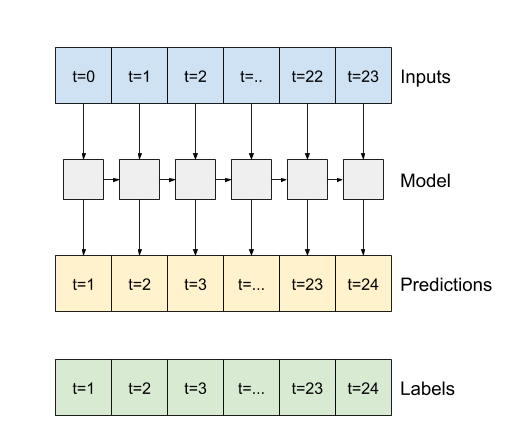
\includegraphics[width=.45\textwidth]{figuras/lstm_many_window.png}
    \caption{Fonte: adaptado de GOOGLE(2025)\cite{tensorflow-structured-data-tutorial}}
    \label{fig:tensorflow1}
\end{figure}

Idealmente, levando em consideração que os dados disponíveis em domínio público possuem granularidade de apenas hora em hora, totalizando 24 medições diárias, é possível que o modelo será ativado para processamento apenas uma vez por hora, permitindo que mais que um modelo utilize o tempo de processamento ocioso.

\subsubsection{Coleta de Dados}

A coleta de dados é realizada através de comunicação I2C com o sensor BME280, utilizando uma taxa de amostragem configurável de 60 segundos por padrão:

\begin{itemize}
    \item \textbf{Inicialização I2C:} O sistema tenta estabelecer comunicação no endereço padrão 0x76
    \item \textbf{Calibração do sensor:} Carregamento dos parâmetros de calibração específicos do chip BME280
    \item \textbf{Validação da conexão:} Leitura de teste para confirmar o funcionamento adequado do sensor
    \item \textbf{Loop de coleta:} Execução em thread separada para não bloquear o servidor web
\end{itemize}

\subsubsection{Processamento de Dados}

Os dados coletados passam por um pipeline de processamento que incluirá filtragem e processamento por modelo de rede neural:

\begin{itemize}
    \item \textbf{Validação inicial:} Verificação de integridade dos dados recebidos do sensor
    \item \textbf{Processamento por rede neural:} Os dados processados serão enviados para um modelo em desenvolvimento para análise preditiva e detecção de padrões climáticos
\end{itemize}

\subsubsection{Armazenamento e Transmissão}

\begin{itemize}
    \item \textbf{Armazenamento em memória:} Cache dos últimos valores para acesso via API REST
    \item \textbf{API REST:} Endpoints padronizados (\texttt{/api/data}, \texttt{/api/status}) para integração com sistemas externos
\end{itemize}

\subsubsection{Interface com o Usuário}

\begin{itemize}
    \item \textbf{Dashboard web:} Interface HTML5/CSS/JavaScript
    \item \textbf{Controle dos sensores:} Botões para iniciar/parar coleta de dados
\end{itemize}

\subsubsection{Inserção no Sistema Operacional}

\begin{itemize}
    \item \textbf{Serviço systemd:} Criação de serviço nativo (\texttt{bme280-station.service}) para inicialização automática
\end{itemize}

O instalador automatizado (\texttt{install.py}) configura todas as dependências, permissões e serviços necessários.

\subsubsection{Arquitetura de Threads}


\begin{itemize}
    \item \textbf{Thread principal:} Servidor Flask para requisições HTTP
    \item \textbf{Thread de coleta:} Loop independente para leitura do sensor
\end{itemize}

O fluxograma do software descrito pode ser visualizado na figura~\ref{fig:fluxograma}. 
Os códigos podem ser encontrados no seguinte repositório: 
\href{https://github.com/lcsgborges/Trabalho-SOE-2025.2/tree/main}{github.com/lcsgborges/Trabalho-SOE-2025.2}.

\begin{figure}[!ht]
    \centering
    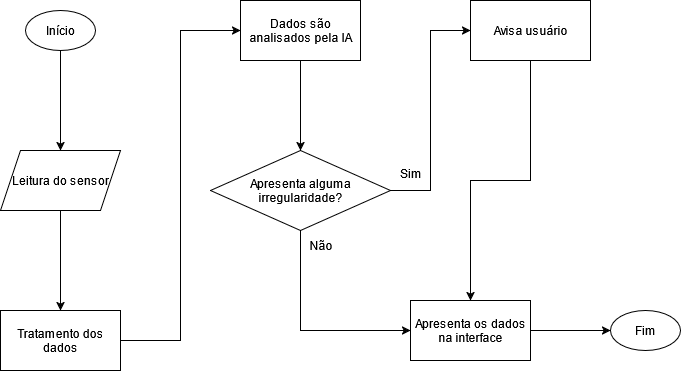
\includegraphics[width=.45\textwidth]{figuras/soe_fluxograma.drawio.png}
    \caption{Fluxograma do software}
    \label{fig:fluxograma}
\end{figure}

